\documentclass[11pt]{article}
\usepackage{comment}
\usepackage{lipsum}
\usepackage{fullpage}
\usepackage{amsmath}
\usepackage{amssymb}
\usepackage{tikz}
\usepackage{tikz-cd}
\usepackage{float}
\usepackage{cleveref}
\usepackage{xifthen}
\usepackage{subfig}
\usepackage
[
        letterpaper,% other options: a3paper, a5paper, etc
        left=1cm,
        right=4cm,
        top=2cm,
        bottom=2cm,
        % use vmargin=2cm to make vertical margins equal to 2cm.
        % us  hmargin=3cm to make horizontal margins equal to 3cm.
        % use margin=3cm to make all margins  equal to 3cm.
]
{geometry}

\setlength{\marginparwidth}{3cm}
\DeclareMathOperator{\dist}{dist}

\begin{document}
\noindent
\large\textbf{Automatic Image Filter Identification} \hfill \textbf{Vision 20/20} \\
\normalsize CS4476, Midterm Project Update \hfill Gokmen, Dumenci, Ye, Lo \\
Prof. Parikh \hfill Georgia Institute of Technology

\section*{Abstract}
Given the prevalence of photo editing and filtering on popular social media platforms such as Snapchat and Instagram, it is becoming more and more difficult for users to identify how the content that they consume everyday have been modified from their original form. Since filtering has become so common, the goal of this project is to give users a means to identify how photos on these platforms are edited and to present a plausible reconstruction of source content.

We propose an end-to-end system that will take an image from the user, identify probabilities for which common image filters were applied to the image, and apply the most likely filter inverse. We present both the filter probabilities and the inverted image to the user. We utilize features in the form of color histograms and scene details to extract a sense of natural color distributions and use neural networks both to determine the probabilities for applied filters and to invert an image given its most likely filter.

% Detection & inversion:
% Roundtrip per-pixel SAD error for 10000 images: 0.05538734147397006
% Baseline per-pixel SAD error for 10000 images: 0.08457501071028349

% Only inversion, known filters:
% Roundtrip per-pixel SAD error for 10000 images: 0.010018754974558564
% Baseline per-pixel SAD error for 10000 images: 0.08495726214719272

From our experiments, we are able to classify images by the filter applied to it (from our predefined set of six Instagram filters) while distinguishing it from natural (unfiltered) images with an accuracy of 60\% to 98\% depending on the characteristics of the filter such as the amount of deviation from the original image. Let $E(I, I')$ be the average per-pixel mean of the sum absolute differences in intensity across all color channels of images $I$ and $I'$ (\textit{Equation 1}). For inverting images given a known filter, we are able to obtain a pseudo-inverse of the image with an average error $E$ of 1\%. End-to-end, our system detects and inverts filters with an average error $E$ of 5.5\% between our output image and the original unfiltered version. In comparison, the baseline error $E$ between filtered and unfiltered images was found to be 8.4\%.

\newcommand{\cimg}[2] {
    \begin{minipage}{#2}\centering \includegraphics[width=#2]{#1}\end{minipage}
}

\section*{Teaser Figure}

\begin{figure}[H]
    \centering
    \begin{tikzcd}
        \cimg{images/gingham.jpg}{2cm} \arrow[r] &
        \text{Filter detector} \arrow{rrr}{\text{Probabilities}}[swap]{\max P(\text{Gingham})} &
         &
         &
        \text{Filter inverter} \arrow[r] &
        \cimg{images/original.jpg}{2cm}
    \end{tikzcd}

    \caption{Architecture overview}
    \label{fig:overview}
\end{figure}


\section*{Introduction}
Filtered photos have become ubiquitous on social media platforms such as Snapchat, Instagram, Flickr, and more. For the casual eye, the subtlety of these filters can make it hard to distinguish between filtered and unfiltered images on social media, leading to a false perceptual model of how natural images look, skewing our expectations about reality. We hope this project will help bring more transparency into how images are often edited by identifying whether a common image filter have been applied to an image, and expose users to the natural state of these images. We believe that transparency in the image editing process is important in raising awareness about deliberate modifications to perceptions of reality, allowing content consumers to enjoy the edited content while being aware of their true nature.

Not to be confused with filters in the computer vision setting, which are often used to better extract information from an image, filters in the social media setting describe a predefined set of modifications to an image that attempts enhance its human visual appeal. Most commonly, these filters come in the form of color balance adjustments and can be represented as tweaks to the color curves of an RGB image. A color curve $f: [0, 255] \to [0, 255]$ is a continuous function that remaps the intensities in each color channel. Modification to the color curve allows the user to non-uniformly boost or decrease color intensities at varying ranges to create various effects such as increasing contrast or creating color shifts (e.g. \cref{fig:color_curve} demonstrates a boost of blues in shadows while decreasing blues in highlights). Some filters also include additional effects such as blurring/sharpening using convolution kernels, the addition of borders, and the application of vignette darkening at the edges.

\begin{figure}[H]
    \centering
    \begin{tikzcd}
        \cimg{images/ampitheatre_before.jpg}{2cm} \arrow[r] &
        \cimg{images/curve.JPG}{2cm} \arrow[r] &
        \cimg{images/curveAfter.JPG}{2cm} \arrow[r] &
        \cimg{images/ampitheatre_after.jpg}{2cm}
    \end{tikzcd}

    \caption{Example of Color Curve Modification on The Blue Color Channel}
    \label{fig:color_curve}
\end{figure}

For the purposes of this project, we limit our scope and define a filter as a pair $(f, g)$ where $f: \mathbb{R}^3 \rightarrow \mathbb{R}^3$ is a function that maps every individual color (consisting of 3 channels each with a real value in the $[0, 1]$ range) to some color in the same range, and $g \in \mathbb{R}^{3 \times 3}$ is a convolution kernel that can be used for blurring and sharpening among other effects. We assume that a filter is applied first by passing each pixel of an image through $f$, and then convolving the image with $g$, extending the edges by repeating the last row and column of pixels as to preserve the shape of the image.

While many commercial filters may also contain additional effects such as borders and vignettes, filters are mostly characterized by how they shift the color curves globally and their blur/sharpen/emboss effects. Therefore, for the scope of this project, we choose filters which does not have these additional effect.

Though our work relates to many other fields of computer vision, such as image denoising and brightening images \cite{Dark}, not much work directly focuses on end to end filter identification or inversion. One publication that we found \cite{IEEE_Inversion} for identification depends heavily on prior knowledge of the camera demosaicing algorithm which is not always readily available. We thus chose to develop our own identification system.

In many of these settings such as image denoising or brightening, the modifications applied to the image (noise, etc.) are either consistent across the dataset or is known a priori. Our task is different from these previous work as our filter functions are unknown, but we have examples of unfiltered \& filtered images. Therefore, we decompose this task of filter inversion into two separate tasks, one is filter identification given an input image and the other is filter inversion given a known filter. Filter identification for an image is a classification task while filter inversion is a regression task estimating the filter inverses.

\section*{Approach}

Our approach splits the end-to-end task of filter inversion into two steps:
\begin{itemize}
    \item Generate a probability vector for possible filters applied to a given image. (Filter classification)
    \item With the image and the probability vector as inputs, apply a learned inverse filter onto the image to recover the unfiltered image. (Filter inversion)
\end{itemize}
% The first generates a probability vector for the possible filters applied to an image. The second takes the most likely filter prediction, and applies the learned inverse filter onto the image to recover the original image.

While there are infinitely many filters possible, popular social media platforms have a few pre-selected filters that are widely used. Therefore, we constrain the scope of our filter inversion by assuming input images were filtered at most once by a filter from a known set. To accurately model a real-world application, our list comprises of the following six popular Instagram filters:

\def\filterimagewidth{3cm}
\begin{figure}[H]
    \centering
    \subfloat[Original image]{\label{fig:original}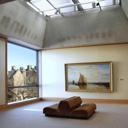
\includegraphics[width=\filterimagewidth]{images/original.jpg}}
    \subfloat[Clarendon]{\label{fig:original}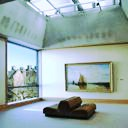
\includegraphics[width=\filterimagewidth]{images/clarendon.jpg}}
    \subfloat[Gingham]{\label{fig:original}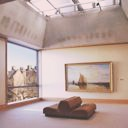
\includegraphics[width=\filterimagewidth]{images/gingham.jpg}}
    \subfloat[Juno]{\label{fig:original}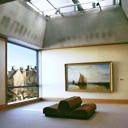
\includegraphics[width=\filterimagewidth]{images/juno.jpg}}\\
    \subfloat[Lark]{\label{fig:original}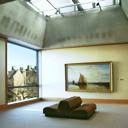
\includegraphics[width=\filterimagewidth]{images/lark.jpg}}
    \subfloat[Gotham]{\label{fig:original}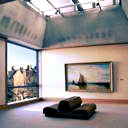
\includegraphics[width=\filterimagewidth]{images/gotham.jpg}}
    \subfloat[Reyes]{\label{fig:original}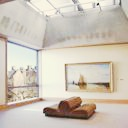
\includegraphics[width=\filterimagewidth]{images/reyes.jpg}}
    \caption{Selected filters}
    \label{fig:filters}
\end{figure}

Given the scant amount of existing literature on the problem of filter identification aside from \cite{IEEE_Inversion}, there were no established processes for filtering large numbers of images using commercial filters. We were prompted to create our own image filtering pipeline. Since Instagram filters are not available outside of their platform, we imitated these filters by manually modifying each color curve. We referenced channel adjustment code from an online article \cite{Instafilters}, which uses \verb|numpy| functions, specifically \verb|linspace| and \verb|interp|, to modify the color curves of each specific channel. We obtained curve parameters for each filter from \cite{Instafilters_tutorial} and passed them onto the channel adjustment code to create an imitation of commercial filters. We then run each imitation filter over our library of unfiltered images to create our dataset.

\subsection*{Filter classification}
Our approach to filter classification takes in an input image and outputs a probability vector for the possible filters applied to the input image. We utilize a neural network model to generate this probability vector from features extracted from the input image.

For feature extraction, because color curves are a major component of many of the popular image filters, we decided to use color histograms to extract global color information from the image. Furthermore, because these color curve modifications are often applied independently in each RGB channel, we create separate color intensity histograms for each color channel and concatenate them together to generate the features for a given image.

Note that this low level data can be augmented with scene and object information, premised on the idea that color distributions are correlated to the subjects and the environment of the image. This augmentation has not yet been incorporated into the pipeline.

Due to the lack of neural network based approaches in the previous work done in this area, we had no intuition on the appropriate complexity required for our models. Therefore, we first experimented with the simplest models with one layer and few neurons, found it performed poorly, and gradually increased complexity until diminishing return on performance occurred.

We utilize Keras \cite{Keras} to create a sequential, feed-forward neural network with varying number of layers at different sizes with the ReLU activation function on the hidden layers. The network ends with a softmax layer to obtain a probability vector. We use the ReLU activation function because it has been consistently shown to provide good performance and training speed for neural networks \cite{ReLU}. We use a cross-entropy loss function and the Adam optimizer \cite{Adam} to train our neural network model.

% TODO(chunlok): Add this back if needed.
One problem we encountered was that because each image passes through 6 different filters and each of these images are in our dataset, we have to ensure that our model has not seen the images before to avoid memorizing previous image color distributions to obtain good results in the testing set. Therefore, we utilize a completely different set of base images for the training and testing set.

\begin{figure}[H]
    \centering
    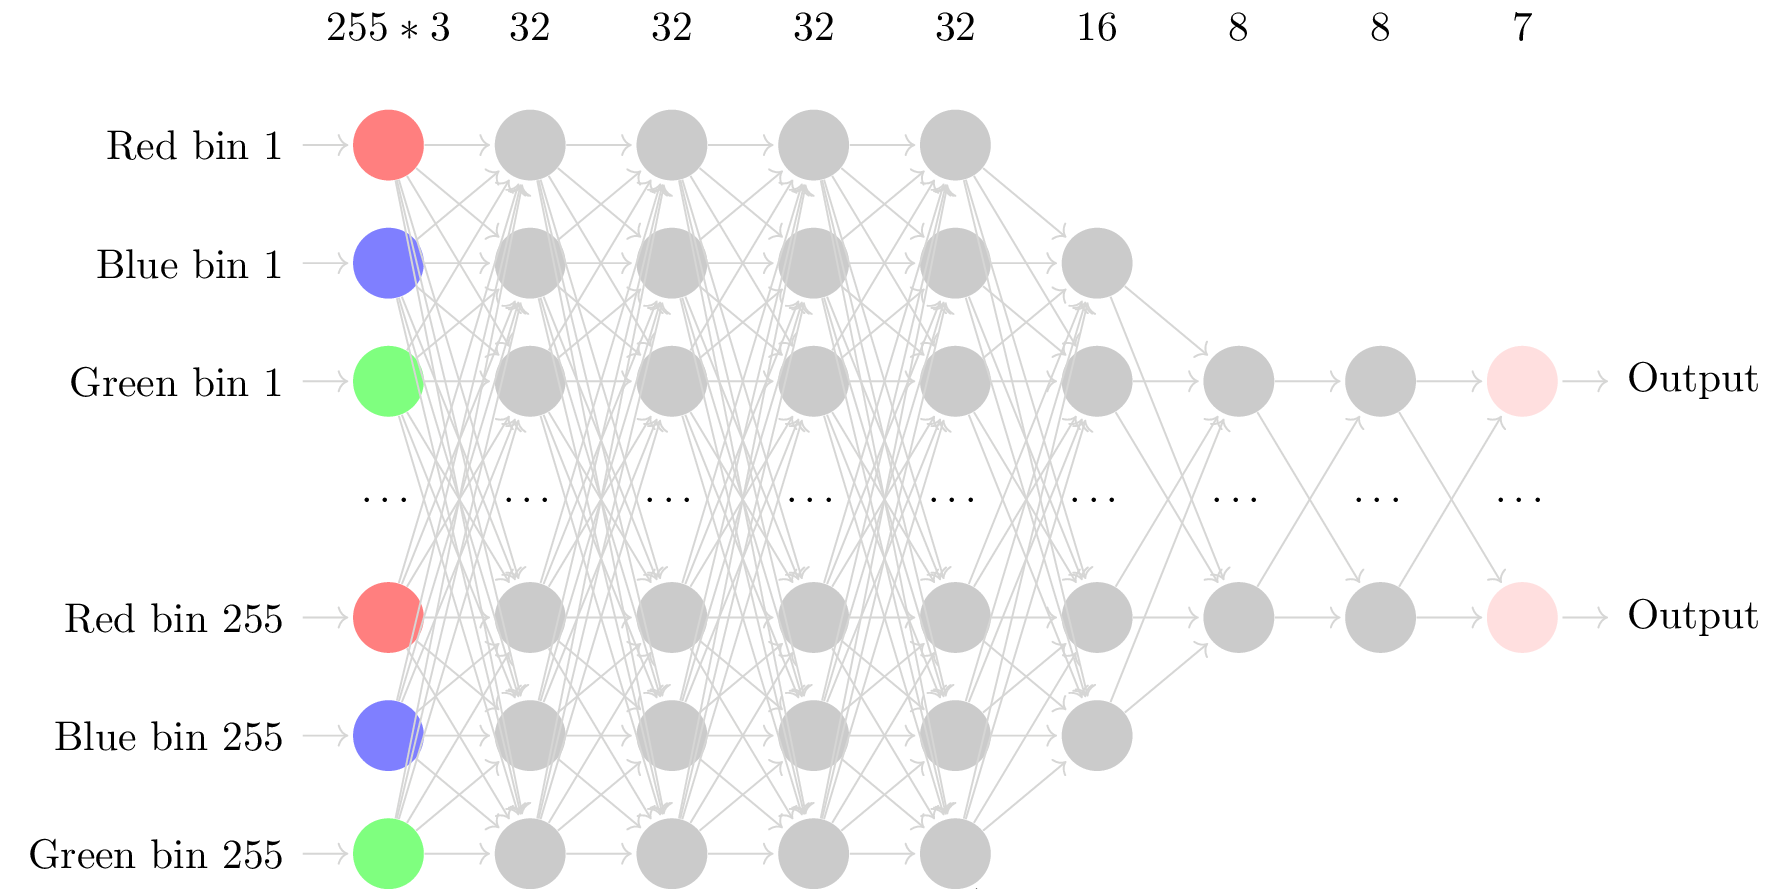
\includegraphics[width=0.6\textwidth]{images/detection-nn.png}
    \caption{Detection NN Architecture}
    \label{fig:detection_nn}
\end{figure}

\subsection*{Filter inversion}
For the inversion of filters, our formalization of a filter is critical. We assume the definition of a filter as a pair $(f, g)$ of a function $f$ that maps colors and a convolution kernel $g$.

With this assumption, we design a set neural networks to approximate the behavior of an inverse filter. The specification of the neural network for one filter $(f, g)$ is such that given a $3 \times 3$ region of pixels, it should be able to learn and undo the convolution $g$ centered at the middle of the square, then learn and apply the inverse of the function $f$, finally outputting the unfiltered color of the middle pixel of the patch.

We set up a neural network model with an input of $3 \times 3 \times 3$ values to represent the RGB colors of the $3 \times 3$ patch, an output of $3$ values to represent the RGB colors of the center pixel, and three hidden layers with $100$ neurons each, to account for potential non-linearities of $f$. We note that since $(f, g)$ are specific to each filter, we will need to train a separate copy of this model for each of our supported filters.

Given a filter, to train a neural network with sufficient data to allow it to generalize properly, we generate 1 million uniformly random $3 \times 3$ RGB patches and apply the filter to all of them. We then store the filtered $3 \times 3$ patches as input $X$ and the center pixel of the unfiltered patches as $y$. Every such $(X, y)$ forms one sample, and we train our neural network on 1 million such samples until validation score plateaus.

Finally, to apply filter inversion to a given image known to be the result of a particular filter $f$, we iterate through the image using a $3 \times 3$ sliding window, and for each step of the iteration we feed the window into the pre-trained neural network corresponding to $f$. The model outputs the predicted unfiltered color of the pixel at the center of the image, which we store in a copy of the image. Repeating this operation over patches centered at each pixel on the image, we reach the predicted unfiltered image.

Note that due to the fact that our model is based on filter functions that we define and implement, it was also possible to attempt to invert all of our filters deterministically that aimed to undo each step of the filter. However, since we do not know the exact function behind the filters used on Instagram, et al. such a method would not be applicable on images filtered using filters whose source code we cannot access, such as images on social media. As a result, we opt for a machine learning method, so that given a sufficiently large dataset of filtered images (alongside their unfiltered counterparts), we can learn to invert any filter that our definition of a filter can represent.

\section*{Experiments}
We perform our experiments using 9000 $128\ \times\ 128$ images from 10 different categories from the MiniPlaces dataset \cite{Places} passed through 6 different filters (\cref{fig:filters}) to create a total dataset of 63000 images (including the original images.) We split these images into 80\% training and 20\% testing sets with assurance that images from the testing set and their filtered derivatives are not in the training set. Therefore, our training set consists of 50400 images while our testing set consisted of 12600 images.

\begin{figure}[H]
    \centering
    \begin{align*}
        \text{7200 images} \times \text{6 filters} + \text{7200 original images} &= \text{50400 training images}\\
        \text{1800 images} \times \text{6 filters} + \text{1800 original images} &= \text{12600 testing images}
    \end{align*}
    \caption{Detection dataset}
    \label{fig:detection_dataset}
\end{figure}

While we experimented with greyscale color histogram at first for its simplicity, the important role of color in filter identification pushed us towards our current feature extraction method. And because filters often modify color curves within the RGB space, we decided to extract three separate color intensity histogram in the RGB channel and concatenate them together as our image feature. We use 255 bins per color channel, which were represented as floats in the range [0, 1]. No meaningful performance gain was observed when increasing the number of bins past 255. Our neural network hyperparameters were tuned through manual search by starting with a simple model and increasing model complexity until no apparent improvements was noticed.

Given the simplicity of features we extract, we expected a simple model to provide comparative performance in the filter identification task. However, after experimentation, adding multiple layers to our model increased our model accuracy by upwards of 8\%. It is possible that applying a filter might affect an image's color histogram in more complex ways than we assumed and increasing the number of layers enabled the network to better understand the effect of filter application on an image's color histogram.

Our final neural network contains four size 32 layers, one size 16 layer, two size 8 layers, and an output softmax layer with 7 nodes, in that order. The network is fully connected and every layer except the last uses \textit{ReLU} activation. The softmax layer produces a probability vector for the predicted filter. An input feature vector for this model contains $255 \times 3 = 765$ features. The main hyperparameter for future experimentation is the number of bins used here, or in general, what we choose to feed into our network. When stepping through increasing bin count, we found performance plateaued at 255 bins.

We trained our neural network classifier for a total of 100 epochs with a batch size of 128 using the Adam optimizer \cite{Adam} and the cross-entropy loss function.

One improvement to note is that we did not utilize validation set (which we should have) during our training process so we do not have an exact measure of overfitting. However, we evaluated our model performance different number of epochs and there were no noticeable increase accuracy from stopping before or going past 100 epochs.

\begin{figure}[H]
    \centering
    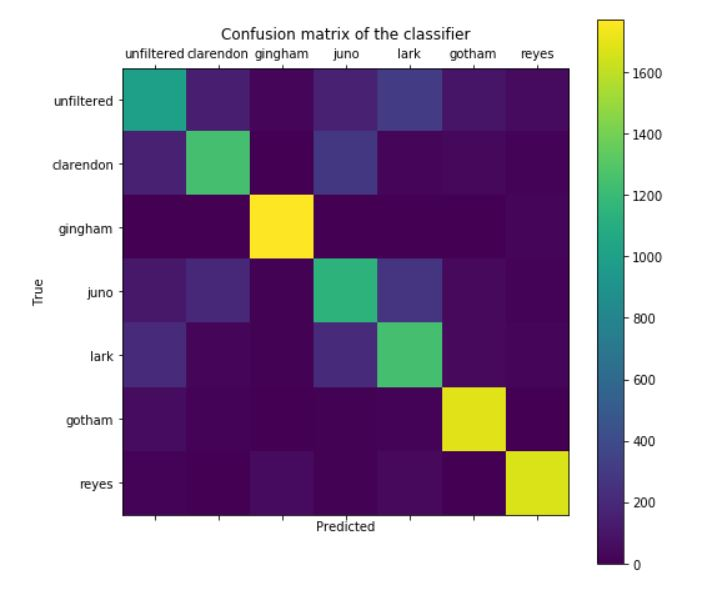
\includegraphics[width=0.6\textwidth]{images/confusionMatrix.jpg}
    \caption{Confusion matrix for detection NN}
    \label{fig:confusion_matrix}
\end{figure}

Our initial approach evaluated our model based on the overall accuracy in the prediction (filter with maximum probability from our probability vector). However, we noticed visually subtler filters naturally had lower identification rates, so we refined our statistics to distinguish success for different filters. We thus also looked at the precision, recall, F1 score, and the confusion matrix to evaluate model performance on individual filters. For comparison, the baseline accuracy of a random classifier is 0.143.

\begin{figure}[H]
    \centering
    \begin{tabular}{|c|c|c|c|c|c|c|c|}
        \hline    & \textit{Identity} & \textit{Clarendon} & \textit{Gingham} & \textit{Juno} & \textit{Lark} & \textit{Gotham} & \textit{Reyes}\\
        \hline \textit{Precision} & 0.635 & 0.760 & 0.944 & 0.625 & 0.647 & 0.879 & 0.921\\
        \hline \textit{Recall}    & 0.554 & 0.693 & 0.984 & 0.638 & 0.695 & 0.939 & 0.929 \\
        \hline \textit{F1}        & 0.591 & 0.725 & 0.964 & 0.631 & 0.670 & 0.908 & 0.925\\
        \hline
    \end{tabular}
    \caption{Detection metrics with 100 bins (over 5 runs) $Acc_{avg} = 0.776, Acc_{random} = 0.143$}
    \label{fig:filter_metrics}
\end{figure}

\begin{figure}[H]
    \centering
    \begin{tabular}{|c|c|c|c|c|c|c|c|}
        \hline    & \textit{Identity} & \textit{Clarendon} & \textit{Gingham} & \textit{Juno} & \textit{Lark} & \textit{Gotham} & \textit{Reyes}\\
        \hline \textit{Precision} & 0.643 & 0.684 & 0.954 & 0.681 & 0.677 & 0.904 & 0.906\\
        \hline \textit{Recall}    & 0.583 & 0.786 & 0.975 & 0.580 & 0.673 & 0.946 & 0.935 \\
        \hline \textit{F1}        & 0.612 & 0.731 & 0.964 & 0.626 & 0.675 & 0.925 & 0.920\\
        \hline
    \end{tabular}
    \caption{Detection metrics with \textbf{255 bins} (over 5 runs) $\mathbf{Acc_{avg} = 0.783}, Acc_{random} = 0.143$}
    \label{fig:filter_metrics}
\end{figure}

\begin{figure}[H]
    \centering
    \begin{tabular}{|c|c|c|c|c|c|c|c|}
        \hline    & \textit{Identity} & \textit{Clarendon} & \textit{Gingham} & \textit{Juno} & \textit{Lark} & \textit{Gotham} & \textit{Reyes}\\
        \hline \textit{Precision} & 0.620 & 0.720 & 0.936 & 0.568 & 0.781 & 0.894 & 0.940\\
        \hline \textit{Recall}    & 0.550 & 0.789 & 0.984 & 0.775 & 0.463 & 0.956 & 0.883 \\
        \hline \textit{F1}        & 0.583 & 0.753 & 0.959 & 0.656 & 0.582 & 0.924 & 0.910\\
        \hline
    \end{tabular}
    \caption{Detection metrics with 300 bins (over 5 runs) $Acc_{avg} = 0.7719, Acc_{random} = 0.143$}
    \label{fig:filter_metrics}
\end{figure}

One interesting trend to examine is the performance difference among different filters. Filters like Gingham, Gotham, and Reyes easily achieve an \textit{F1 score} of over 0.9 while other filters’ \textit{F1 scores} all fall below 0.8. We believe that this is attributed to how large of a visual effect these filters have on the output image, as illustrated in \cref{fig:filters}.

These filters are quite obvious when compared side by side to the original filter, or more technically, consider the difference in tone shifts between each of these different filters. We believe the tone shifts within Gingham, Gotham, and Reyes appear more unnatural (Gingham and Gotham gives a red tint while Reyes gives an overall white tint to the image) whereas Juno, Lark, and Clarendon appear more natural by adding blueish, greenish, or yellowish lighting to the image, making them harder to distinguish from an unfiltered photo.

For the accuracy of our filter inverter, if the filter of an image is known, the average per-pixel sum of absolute difference (SAD) error summed across three RGB channel for 10000 images was 0.010 whereas the baseline per-pixel SAD error without inversion for 10000 images: 0.085. We are currently working on getting more comprehensive experimentation results on the performance of our filter inverter.

Laying groundwork for improving the system, we also investigated how scene information could be used, hoping that scene knowledge encode expectations about what colors compose an image. Initial experiments of a separate system to prove this hypothesis were done using a pretrained VGG16 Keras model on Places365 \cite{Places}, which, as the name suggests, provides scene probabilities among a set of common scenes $S$. Using the same filtered image creation pipeline, we built a corpus of expected distributions for a given scene under any filter. In the training step of this system, we ran through 2000 arbitrary scenes and ran color binning with 25 bins per color, under each filter. Each feature vector $F$ is then length 75. These histograms were distributed across detected scenes according the probability vector given provided by the model, and saved to a final corpus of shape $(|\text{filters}| + 1) \times |S| \times |F|$ . The saved feature representation for a given filter and scene was a normalized sum of the distributions that contributed towards it.
A prediction of a filter in this system is done simply by running scene detection on the input and referencing the appropriate set of features weighted according to the scene probability vector. Euclidean distance of expected features and input features was used to approximate error, put through softmax to create probabilities for which filter was applied. The distribution of our input should best match a representative distribution for the detected scene under the input's filter. Trained with a corpus of both 200 and 2000 images, the system outputs correct filter as one of its top two candidates $70\%$ of the time. In both cases, scene information sufficed to predict some of the more apparent filters discussed above, but was limited. It's clear that scene information is useful, and will be incorporated into the network as another feature.

\section*{Qualitative Results}

\subsection*{Examples}
\begin{figure}[H]
    \centering
    \subfloat[Original image]{\label{fig:original}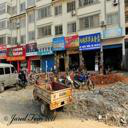
\includegraphics[width=\filterimagewidth]{images/0.png}}
    \subfloat[Filtered image]{\label{fig:original}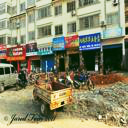
\includegraphics[width=\filterimagewidth]{images/filtered_0.png}}
    \subfloat[Inverted image]{\label{fig:original}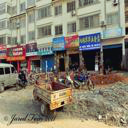
\includegraphics[width=\filterimagewidth]{images/inverted_0_lark.png}}
    \caption{End-to-end \textit{Lark} example}
    \label{fig:filters}
\end{figure}

\begin{figure}[H]
    \centering
    \subfloat[Original image]{\label{fig:original}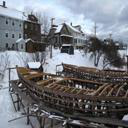
\includegraphics[width=\filterimagewidth]{images/17.png}}
    \subfloat[Filtered image]{\label{fig:original}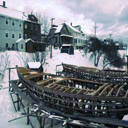
\includegraphics[width=\filterimagewidth]{images/filtered_17.png}}
    \subfloat[Inverted image]{\label{fig:original}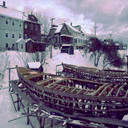
\includegraphics[width=\filterimagewidth]{images/inverted_17_clarendon.png}}
    \caption{End-to-end \textit{Clarendon} example}
    \label{fig:filters}
\end{figure}

\begin{figure}[H]
    \centering
    \subfloat[Original image]{\label{fig:original}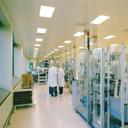
\includegraphics[width=\filterimagewidth]{images/2.png}}
    \subfloat[Filtered image]{\label{fig:original}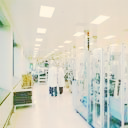
\includegraphics[width=\filterimagewidth]{images/filtered_2.png}}
    \subfloat[Inverted image]{\label{fig:original}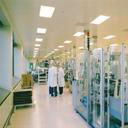
\includegraphics[width=\filterimagewidth]{images/inverted_2_reyes.png}}
    \caption{End-to-end \textit{Reyes} example}
    \label{fig:filters}
\end{figure}

\subsection*{Failure cases: Filter Detection Failures}
\begin{figure}[H]
    \centering
    \subfloat[Original image]{\label{fig:original}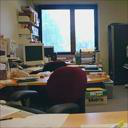
\includegraphics[width=\filterimagewidth]{images/4.png}}
    \subfloat[Filtered image]{\label{fig:original}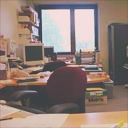
\includegraphics[width=\filterimagewidth]{images/filtered_4.png}}
    \subfloat[Inverted image]{\label{fig:original}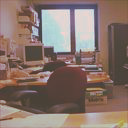
\includegraphics[width=\filterimagewidth]{images/inverted_4_gingham.png}}
    \caption{End-to-end \textit{Gingham} example}
    \label{fig:filters}
\end{figure}

\begin{figure}[H]
    \centering
    \subfloat[Original image]{\label{fig:original}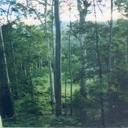
\includegraphics[width=\filterimagewidth]{images/43.png}}
    \subfloat[Filtered image]{\label{fig:original}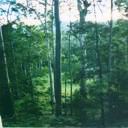
\includegraphics[width=\filterimagewidth]{images/filtered_43.png}}
    \subfloat[Inverted image]{\label{fig:original}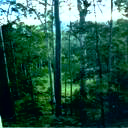
\includegraphics[width=\filterimagewidth]{images/inverted_43_juno.png}}
    \caption{End-to-end \textit{Juno} example}
    \label{fig:filters}
\end{figure}

\begin{figure}[H]
    \centering
    \subfloat[Original image]{\label{fig:original}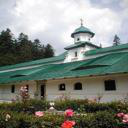
\includegraphics[width=\filterimagewidth]{images/22.png}}
    \subfloat[Filtered image]{\label{fig:original}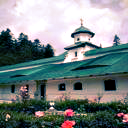
\includegraphics[width=\filterimagewidth]{images/filtered_22.png}}
    \subfloat[Inverted image]{\label{fig:original}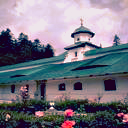
\includegraphics[width=\filterimagewidth]{images/inverted_22_gotham.png}}
    \caption{End-to-end \textit{Gotham} example}
    \label{fig:filters}
\end{figure}

\section*{Conclusion and Future Work}
For filter detection, we already have promising performance with simple color histograms as features. From our experiments, we are able to achieve an average accuracy of 78\% across a set of 6 filters, each with a different effect on the color curves of our image.

For filter inversion, our trained models can invert known filters with an error $E$ (Equation 1) of 1\%, averaged across all 6 filters. These approaches combined, our end-to-end model is able to achieve an error $E$ of 5.5\%, which compares to the error $E'$ of 8.4\% between filtered and unfiltered images.

% I think the below sentence sounds like a rehash, not a conclusion.
% The application of this project is to give users a better means to identify how content they consume on social media platforms are edited and present them with the original content as social media platforms and thus filter edited content become more and more prevalent in our world. This system that we present takes in an image without knowing whether a filtered has been applied and produces not only a probability vector for which possible filter has been applied and provides an attempt at inverting the filter. Through utilizing color channel histograms as features of our image and using Neural Networks to model the classification task and the inversion filter. From our experiments, we are able to achieve an average accuracy of 0.78 across 6 different filters, each with a different effect on the color curves of our image. In total, our current system achieves an average of 2\% error per pixel when comparing our system output to an unfiltered image.
We believe our system can improve both its filter identification and inversion. We will continue experimenting with different features to feed into the detection models such as histograms in HSV space instead of RGB space, which might quantify perceptual changes to images better than RGB histograms. As mentioned, the color distributions of an image are a function of the subjects and the environment of the image in addition to the filter applied. We plan to incorporate explicit scene information to the model, which we predict will help the model establish a baseline for each scene, further simplifying the classification of the perturbations on the image caused by a filter.

Supporting our intuition, our preliminary experiments with filter identification using scene information perform better than a random baseline as described in \textit{Experiments}, meaning there is latent color information embedded in a scene.

For further granularity, an alternative route we will investigate is running object detection with Mask R-CNN \cite{MaskRCNN} and running filter detection with objects as features. The objects will then vote on a global filter, using weights derived from their sizes and prediction confidence. As a similar (but more complex) idea to the scene approach, we expect this method to give us the best results as granular objects are expected to have the most uniform color distributions across instances. However, we expect roadblocks due to difficulty of modifying the intensive net required for MaskRCNN.

To improve filter inversion, the next steps will be removing the discrete filter selection step between the detection and inversion models, directly providing the inversion subsystem with the filter probability vector. This should allow the inversion model to compute more nuanced inversions by combining the inversion of several filters depending on the certainty of the classifier. The result should allow us to create a more generic filter inverter which can take in additional features to enhance the inversion results.

\begin{thebibliography}{9}
\bibitem{IEEE_Inversion}
C. Chen and M. C. Stamm, ``Image filter identification using demosaicing residual features,'' 2017 IEEE International Conference on Image Processing (ICIP), Beijing, 2017, pp. 4103-4107.

\bibitem{Keras}
F. Chollet and others, ``Keras'', GitHub, 2015.

\bibitem{Adam}
D. P. Kingma and J. Ba, ``Adam: A Method for Stochastic Optimization'', 3rd International Conference for Learning Representations, San Diego, 2015.

\bibitem{Instafilters}
M. Pratusevich, ``Instagram Filters in 15 Lines of Python'', Practice Python, 2016. \textit{Retrieved from URL, https://www.practicepython.org/blog/2016/12/20/instagram-filters-python.html}.

\bibitem{Instafilters_tutorial}
GraphixTV, ``Instagram Filter Effects Tutorials'', YouTube, 2017. \textit{Retrieved from URL,
https://www.youtube.com/playlist?list=PLESCEzav4FyfUIi0RHMkNbQI-9JVr4kJc}

\bibitem{MaskRCNN}
H. Kaiming, G. Gkioxari, P. Doll{\'{a}}r and R. B. Girshick, ``Mask R-CNN'', Facebook AI Research, 2018.

\bibitem{Places} B. Zhou, A. Lapedriza, A. Khosla, A. Oliva, and A. Torralba ``Places: A 10 million Image Database for Scene Recognition'', IEEE Transactions on Pattern Analysis and Machine Intelligence, 2017.

\bibitem{Dark}
C. Chen, C. Chen, J. Xu, and V. Koltun, ``Learning to See in the Dark'', CVPR, 2018.

\bibitem{ReLU}
R. K. Srivastava, J. Masci, F. Gomez and J. Schmidhuber, ``Understanding Locally Competitive Networks'', ICLR, 2015.

\end{thebibliography}
\end{document}
